\section{Stations in depth} \label{sec:stations}
\src{DockStation}s are the most complex classes, or modules, of the framework. Some of the stations offer fine tuning that could be interesting for the more ambitious projects, the goal of this chapter is to show some of the these advanced configuration options. In no way can this chapter replace studying the API documentation and the source code itself. Before reading this chapter you should read about the Basics (page \pageref{sec:basics}), it offers a nice overview of the stations.

\subsection{ScreenDockStation}
This station packs its children into free floating panels. These panels are called windows, and can be moved and resized by the user.

\subsubsection{Window type}
The windows (of type \src{ScreenDockWindow}) are usually \src{JDialog}s. The reason for this is, that a \src{JDialog} is guaranteed to float over its parent frame.
In some applications however a \src{JDialog} is not the correct tool, in these cases a client can implement custom \src{ScreenDockWindow}s or reuse and configure some of the existing windows. For this to happen a client has to implement a \src{ScreenDockWindowFactory} and use the property key \linebreak \src{ScreenDockStation.WINDOW\_FACTORY} to set it. The factory may be an instance of \src{DefaultScreenDockWindowFactory} with non-default settings.

\classbox{
\begin{itemize}
 \item \src{ScreenDockDialog} is the default window.
 \item \src{ScreenDockFrame} is exactly the same as the dialog, just using a \src{JFrame} instead.
 \item \src{InternalDockDialog} is a dialog that can appear on a \src{JDesktopPane}. If using this window, the client should also install an \src{InternalFullscreenStrategy}.
 \item \src{DefaultScreenDockWindowFactory} offers several methods to configure the dialog, including an option to show the OS dependent controls.
\end{itemize}
}

\infobox{New implementations of \src{ScreenDockWindow} should be subclasses of \src{AbstractScreenDockWindow}. This class offers everything a window needs except the
window-container itself.}

Should a client implement a completely new \src{ScreenDockWindow}, then it will be required to implement a matching \src{ScreenDockFullscreenStrategy}.
Accessing the \src{MagnetController} and use its \src{start} method will allow the new window to feature attraction and stickiness.

\subsubsection{Window configuration}
The look and behavior of each default \src{ScreenDockWindow} can be configured, some of the available options are:
\begin{itemize}
 \item Whether the window is transparent
 \item Whether the window can be resized by the user
 \item To move if the title of a \src{Dockable} is dragged
 \item What kind of border to paint
\end{itemize}
All these options are set by the \src{ScreenDockWindowConfiguration}, which really is just a factory creating new instances of \src{WindowConfiguration}. The factory can be set using the property key \src{ScreenDockStation.WINDOW\_CONFIGURATION}.

\warningbox{Do not subclass \src{WindowConfiguration}. Use the \src{set}-methods to change its properties.}

\subsubsection{Stickiness and attraction}
What happens when a window is dragged near another window? Or if two windows touch each other and one of them is dragged away? The framework offers some special behavior in these cases:
\begin{itemize}
 \item A window dragged near another window can be \emph{attracted} to the fixed window. The dragged window will move itself a little bit such that the sides of the windows touch each other.
 \item A window dragged away from a neighbour can be \emph{sticking} to the neighbour. If one window is dragged, the neighbours are automatically dragged as well.
\end{itemize}
The exact behavior of each window is defined by the \src{AttractorStrategy}. Clients can set up their own strategy by using the property key \newline \src{ScreenDockStation.ATTRACTOR\_STRATEGY}.

\classbox{
The actual implementation of attracting and sticking windows is provided by the \src{MagnetStrategy}, which can be replaced using the property key \src{ScreenDockStation.MAGNET\_STRATEGY}.
Clients providing their own \src{MagnetStrategy} may be interested in using the \src{StickMagnetGraph}, a class that analyzes the layout of the windows and their dependencies. }

\subsubsection{Fullscreen}
Since a standard \src{JDialog} can not be maximized, and the \src{ScreenDockWindow}s usually are \src{JDialog}s, the framework must find out on its own when a window is maximized. This property, also called ``fullscreen'', is defined by the interface \src{ScreenDockFullscreenStrategy}. Replacing it usually makes little sense, but it can be done using the property key \src{ScreenDockStation.FULL\_SCREEN\_STRATEGY}.

\designbox{It seems like there can be only one definition of ``fullscreen''. But because the framework does nowhere enforce that a \src{ScreenDockWindow} indeed is a real window, it does neither define what a ``screen'' could be. And it is really hard to globally define ``fullscreen'' when there is no definition of ``screen''. }

\subsubsection{Drop size}
What happens when a \src{Dockable} is dropped onto a \src{ScreenDockStation}? It is put into a window, but how big should this window be? The default behavior of the framework is to look at the current size of the \src{Dockable}, and keep that size. Another solution could be to make sure the \src{Dockable} has its preferred size. A client can change the default behavior by implementing a \src{ScreenDropSizeStrategy}, and installing it using the property key \linebreak \src{ScreenDockStation.DROP\_SIZE\_STRATEGY}.

\subsection{SplitDockStation}
The \src{SplitDockStation} organizes its children in a layout that might look at first glance like a grid, but in reality is a binary tree. Each \src{Dockable} is a leaf in that tree. Any node has an orientation (horizontal or vertical) telling how its children are aligned, and a \src{divider} property telling the relative size of the children. Users modify the tree through drag and drop, but clients can access and modify the tree programatically.

\subsubsection{The tree}
The layout-tree is represented by objects of type \src{SplitNode}. Each node can be seen as a rectangle on the screen, and the children of each node must be within that rectangle. To be more precise, there are four different types of nodes in the tree:

\begin{itemize}
 \item The \src{Root} node really has no special meaning, it is just a wrapper around another node promoting that other node to be the true root.
 \item A \src{Node} has exactly two children. The node has an orientation that tells how the children are aligned, and it has the \src{divider} property, a \src{double} between \src{0} and \src{1.0}, telling the size of the first child in respect to the size of the node itself.
 \item A \src{Leaf} is a wrapper around a \src{Dockable}.
 \item Finally a \src{Placeholder} is not visible to the user. When a \src{Leaf} is removed from the tree a \src{Placeholder} may remain. This placeholder can later be converted back into the \src{Leaf} that was removed.
\end{itemize}
Clients can access the tree by calling \src{SplitDockStation.getRoot}.

\warningbox{Usually modifying the tree directly is a bad idea. When modifying the tree, be aware of:
\begin{itemize}
 \item The tree does not validate itself, if a client creates an invalid tree the application will simply show a very strange layout or start throwing exceptions.
 \item Removing or adding branches to the tree does not automatically remove or add \src{Dockable}s.
\end{itemize}
}

Instead of accessing the tree directly, and perhaps causing a lot of damage, clients can make use of the class \src{DockableSplitDockTree}. A client can create a new \src{SplitDockTree} and call \src{SplitDockStation.dropTree} to replace the current layout of the station.

\infobox{\src{SplitDockTree} may look very hard to use, many methods need to be called just to build a simple tree. But there are some advantages that should be considered:
\begin{itemize}
 \item This class is very safe to use, it is nearly impossible to create an invalid tree with it.
 \item The tree is built from bottom to top, it is an ideal tool to have different methods build and deliver different branches of the tree.
 \item A \src{SplitDockGrid} can be converted into a \src{SplitDockTree}
\end{itemize}
}

\subsubsection{Divider}
Between each two \src{Dockable}s, there is a little gap. The user can grab this gap with the mouse and move it around. For the very unlikely case that a client needs to modify this behavior, there exists the interface \src{SplitDividerStrategy}. The interface itself really does not do much, it gets a \src{Component} and there are some suggestions in the API documentation of what the interface should do with that \src{Component}. The divider strategy is changed by using the property key \src{SplitDockStation.DIVIDER\_STRATEGY}.

\subsubsection{LayoutManager}
There are many actions a user can perform: making a \src{Dockable} ``fullscreen'' (the station hides all other children), drop a new \src{Dockable}, adjust the sizes of the children, or adjust the size of the entire station. In older versions code that reacted to or implemented these actions was either part of the \src{SplitDockStation} itself, or of the \src{SplitNode}s. New developments showed, that it was nearly impossible to modify the behavior. To solve the issue \src{SplitLayoutManager} was introduced, now these user actions are forwarded to one of the methods of \src{SplitLayoutManager}, and the manager may decide either to call the old code, or to chose a custom solution. It is unlikely that a client ever needs to change the \src{SplitLayoutManager}, but it can be done with the property key \src{SplitDockStation.LAYOUT\_MANAGER}.

\subsection{StackDockStation}
The \src{StackDockStation} acts like a \src{JTabbedPane}, only one of its children is visible at any time. The look of this station highly depends on the current \src{DockTheme}. Each theme defines a \src{StackDockComponent}, and this object is responsible for creating, painting and layouting the tabs. While the \src{BasicTheme} makes use of a \src{JTabbedPane}, all the other themes make use of a class called \src{CombinedStackDockComponent}. This means that tabs usually have the same behavior, even if they look differently.

\warningbox{Much of what is written in this chapter does not apply to the \src{BasicTheme}, because the abilities of the \src{JTabbedPane} are very limited compared to the abilities of \src{CombinedStackDockComponent}.}

\subsubsection{TabPane}
The class \src{CombinedStackDockComponent} is shared by the \src{EclipseTheme}, \linebreak \src{BubbleTheme} and \src{FlatTheme}. While the class is responsible for painting and layouting tabs, the real magic happens in its superclass \src{AbstractTabPane}, which implements the interface \src{TabPane}. \src{TabPane} is completely independent from \src{StackDockStation}, and only \src{CombinedStackDockComponent} brings the two modules together.

\designbox{\src{TabPane} does not need to know about \src{StackDockStation}, it just has to offer some methods to add and remove tabs. This allows to make a separation: \src{TabPane} is responsible for painting tabs, \src{StackDockStation} is responsible for deciding which tabs exist.}

\src{TabPane} was designed to show \src{Dockable}s, and as a result it has much more features than a \src{JTabbedPane}. To understand the next chapters, it is certainly a good idea to have an overwiev of the different parts of a \src{TabPane}.

Figure \ref{fig:tabsOverview} shows some tabs how they could appear in any application. The items to the left are called \emph{tabs}, while the button on the right side are part of the \emph{info-component}.

\begin{figure}[h!]
  \centering
    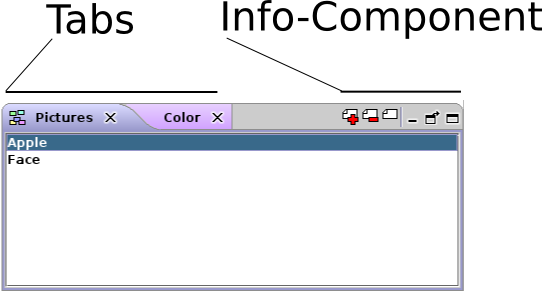
\includegraphics[width=0.5\textwidth]{stations/tabsOverview}
  \caption{A \src{TabPane} with enough space shows some tabs, and some \src{DockAction}s that are associated with the currently selected \src{Dockable}.}
  \label{fig:tabsOverview}
\end{figure}

Figure \ref{fig:smallTabs} shows what happens if there is not enough space to show all tabs. An additional component shows up, a menu called \emph{tab-menu} allows the user to select the tabs that are not visible.

\begin{figure}[h!]
  \centering
    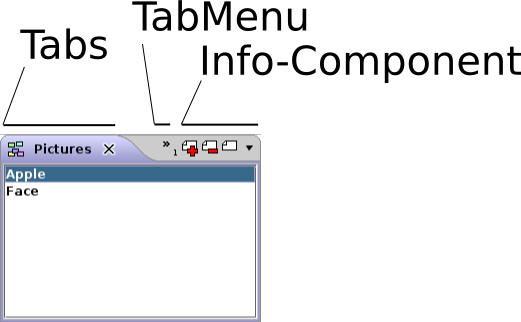
\includegraphics[width=0.5\textwidth]{stations/smallTabs}
  \caption{A \src{TabPane} that has not enough space can show a \emph{tab-menu}, this menu allows the user to select \src{Dockable}s that are otherwise not accessible.}
  \label{fig:smallTabs}
\end{figure}

Finally figure \ref{fig:tab} shows a single tab. Each tab can contain an icon, some text, and perhaps some buttons.

\begin{figure}[h!]
  \centering
    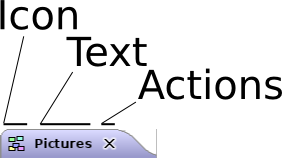
\includegraphics[width=0.25\textwidth]{stations/tab}
  \caption{A single tab shows the title information of the \src{Dockable} it is associated with, including some of its \src{DockAction}s.}
  \label{fig:tab}
\end{figure}

\classbox{A \src{TabPane} is nearly the same as a \src{JTabbedPane}. The tabs are represented by the interface \src{Tab}, the menu showing inaccessible \src{Dockable}s are of type \src{TabMenu}. An additional info-component of type \src{LonelyTabPaneComponent} shows \src{DockAction}s.

Clients that want to implement a new \src{TabPane} should subclass either \src{AbstractTabPane} or \src{CombinedStackDockComponent}.}

\subsubsection{Tab content}
What information should a tab show? Well, the icon and the title-text of the \src{Dockable} seems like a good idea. But since many tabs have to share limited space, some developers may decide it would be a good idea to limit the length of the text, or not to show any icons. The \src{TabContentFilter} allows clients to override the default icon, text and tooltip of a tab. A new \src{TabContentFilter} can be installed by using the property key \src{StackDockStation.TAB\_CONTENT\_FILTER}.

\subsubsection{Tab configuration}
When a tab runs out of space some drastic actions have to be performed. For example the tab could stop painting its icon, this gives at least 20 free pixels. Or it could stop painting its title text, to make sure the icon remains visible. What exactly happens in such a situation depends on the \src{TabConfiguration}, and this configuration is created by the factory \src{TabConfigurations}.

Clients can change the configuration using the property key \linebreak \src{StackDockStation.TAB\_CONFIGURATION}.

\subsubsection{Header layout}
Like a \src{java.awt.Container} using a \src{LayoutManager}, a \src{TabPane} makes use of a \src{TabLayoutManager}. The \src{TabLayoutManager} defines the size and location of all tabs, menu and info-component. The \src{TabLayoutManager} receives a \src{TabPane} and by calling methods like \src{putOnTab} it can tell the \src{TabPane} how to present the \src{Dockable}s. Clients can set a custom layout manager using the property key \src{TabPane.LAYOUT\_MANAGER}.

\classbox{The default implementation of \src{TabLayoutManager} is \src{MenuLineLayout}. This class uses a factory called \src{MenuLineLayoutFactory} to configure some of the details of the layout. The method \src{createOrder} is of special interest, it returns a \src{MenuLineLayoutOrder} which tells order and weight of tabs, menu and info-component. }

\subsection{FlapDockStation}
The \src{FlapDockStation} shows a line of ``buttons'', if clicking one a window opens showing a \src{Dockable}. At any time, only one \src{Dockable} can be shown.

\subsubsection{Button content}
The buttons consists of different parts, as can be seen in figure \ref{fig:flap}. These parts have different jobs:
\begin{description}
 \item[Knob] The knob provides an empty area where the user can grab the button. It ensures that drag and drop is always possible.
 \item[Icon] That is just the icon of the \src{Dockable}.
 \item[Text] The title-text of the \src{Dockable}.
 \item[Children] If the button represents a \src{DockStation}, then the button can show actions to quickly select one of the children of the \src{DockStation}.
 \item[Actions] \src{DockAction}s associated with a \src{Dockable} can be shown on the button as well.
\end{description}

\begin{figure}[h!]
  \centering
    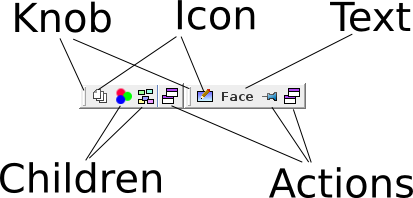
\includegraphics[width=0.5\textwidth]{stations/flap}
  \caption{Two flap-buttons. The left button shows a stack of \src{Dockable}s, while the right button shows a single \src{Dockable}.}
  \label{fig:flap}
\end{figure}

Which of these elements show up depends on the class \src{ButtonContent}. It offers some conditions with which the framework can decide whether to show an element or not. A \src{ButtonContent} can be set using the property key \src{FlapDockStation.BUTTON\_CONTENT}.

\infobox{There are several default setups for \src{ButtonContent} available as constants in \src{ButtonContent} itself. The conditions are modeled by \src{ButtonContentCondition}, an interface that can be implemented by clients.}

\classbox{The buttons are \src{DockTitle}s, the default \src{DockTheme}s all use \src{BasicButtonDockTitle} as button. Clients can install custom buttons by accessing the \src{DockTitleManager} and using the key \src{FlapDockStation.BUTTON\_TITLE\_ID}.}

\subsubsection{Button actions}
The flap-button can show \src{DockAction}s that are associated with the \src{Dockable}. But since space is a limited resource, usually not all actions are shown. The default behavior is to show only actions which are annotated with \linebreak \src{ButtonContentAction}. Clients may change the behavior by implementing the interface \src{ButtonContentFilter} and installing it using the property key \src{FlapDockStation.BUTTON\_CONTENT\_FILTER}.
